% !Mode:: "TeX:UTF-8"

\chapter[模拟退火算法]{模拟退火算法}
\section{模拟退火算法介绍}
   模拟退火算法(Simmulated Annealing Method),简称SA,由Kirpatrick et al\cite{obsa}
在Metropolis et al的基础工作之上提出,是一种通用概率算法,用来在固定时间内寻求一个大的搜寻空间内找到的最优解。
Metropolis当时已经实现了单机和并行的算法,能够解决大部分非常困难的组合优化问题。

    模拟退火算法基于统计力学和组合优化的类比问题。模拟退火算法来源于固体退火原理。退火一词来源于将固体加温高温,
再让其按照特定速率冷,目的是增大晶体的体积,减少晶体的缺陷,此过程中原子会离开原来的位置,随机在其他位置中移动。
冷却至特定温度时,此时系统能够到达稳定状态(系统的内能降到最低),系统内的粒子逐渐有序。将此原理应用到统计学上,将
搜索空间内每一点想象成空气内的分子;分子的能量,就是它本身的动能;搜索解空间的每一点,也像空气分子一样带有"能量“,以表示
对解的合适程度。算法以搜索空间内的一个任意点作为起始点,每一步先选择一个”邻居“,然后判断邻居是否符合特定期望,如果不符合
则以特定概率移动到“邻居"。模拟退火算法可以依概率得到全局最优解。

   将模拟退火算法建立在物理模型上有两个条件,第一,当物体的温度足够高时,系统的动能状态可以自由变化,可以在能量表面自由
地移动或者无规则运动,也就是能够自由地选择可行解;第二,当物体的温度降低时,系统的动能将收到限制,并逐渐的向低能量的区域
集中,在每一次的迭代过程中,都是一目前解作为中心然后随机产生新的临近解,当临近解来取代目前解,如果临近解不够好,利用概率
函数和控制温度的参数来判断是否接受新解,这也是模拟退火算法具有了脱离了居于最佳解,通过降温的计划来控制解的收敛速度,当温度
下降,获取较差接的概率也会变得越来越小,当温度降到最低点,容易获取到最佳解而收敛,如图~\ref{fig:sa1}

\begin{figure}[htbp]
\centering
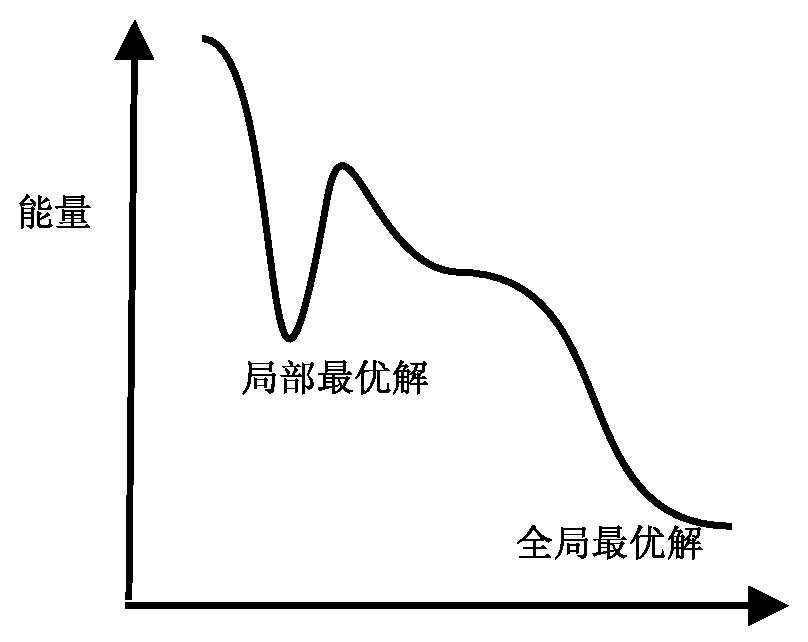
\includegraphics[width=0.6\textwidth]{sa1}
\caption{模拟退火算法示意图}\label{fig:sa1}
\vspace{\baselineskip}
\end{figure}


   根据Metropolis的理论,在温度T时,粒子趋于平衡的概率为$P(T)=e-ΔE/(kT)$,其中E为温度T时的内能,ΔE为内能变化量,k
为常数。在解决组合优化问题时,内能E模拟为目标值F,温度T模拟为参数t,算法由初始解$F_{init}$和控制参数初值t开始,从初始解开开始
重复“产生新解$\rightarrow$计算与目标函数的差$\rightarrow$接受或舍弃”的算法,t值同时逐步衰减,算法结束时的获得到的解即所得近似
最优解。整个退火过程由冷却进度表控制,初始控制参数值t及其衰减因子$Δt$、t值的使用次数L和停止条件S\cite{Zhouping}。 

    总的来说,模拟退火算法可以分解为解空间、目标函数和初始解三部分。模拟退火算法可以分为四个步骤:1 创造新解。有特定的产生函数从当前解产生一个新解,产生方法有元素变换,反置等等; 2
计算差值。对新解和目标函数进行差值运算;3 判断是否接受新值。 判断依据见上述步骤第六步;4 当新解被接受了,用新解替代当前解。

    算法的基本步骤如下:
\begin{enumerate}
\item  初始化:初始化温度T $\infty$,初始解状态S,每个t值的步数L
\item  对k=1,\ldots, L重复第3到第6步
\item  产生新解$S^{'}$
\item  计算增量$\triangle^{'}=C(S^{'})-C(S)$,其中C()为评价解的函数
\item  若$\triangle^{'}<0$则接受$S^{'}$作为新的当前解,否则以概率$exp(-\triangle^{'}T$接受
$S^{'}$作为新的当前解.
\item  如果满足终止条件S,或者到达t值的步数L,则当前解作为最优解输出。终止条件S通常为连续若干个新解都没有
被接受。
\item  t减1,且$T>0$,然后转第2步。
\end{enumerate}

整个模拟退火算法流程图如图~\ref{fig:simulatedannealing}所示

\begin{figure}[htbp]
\centering
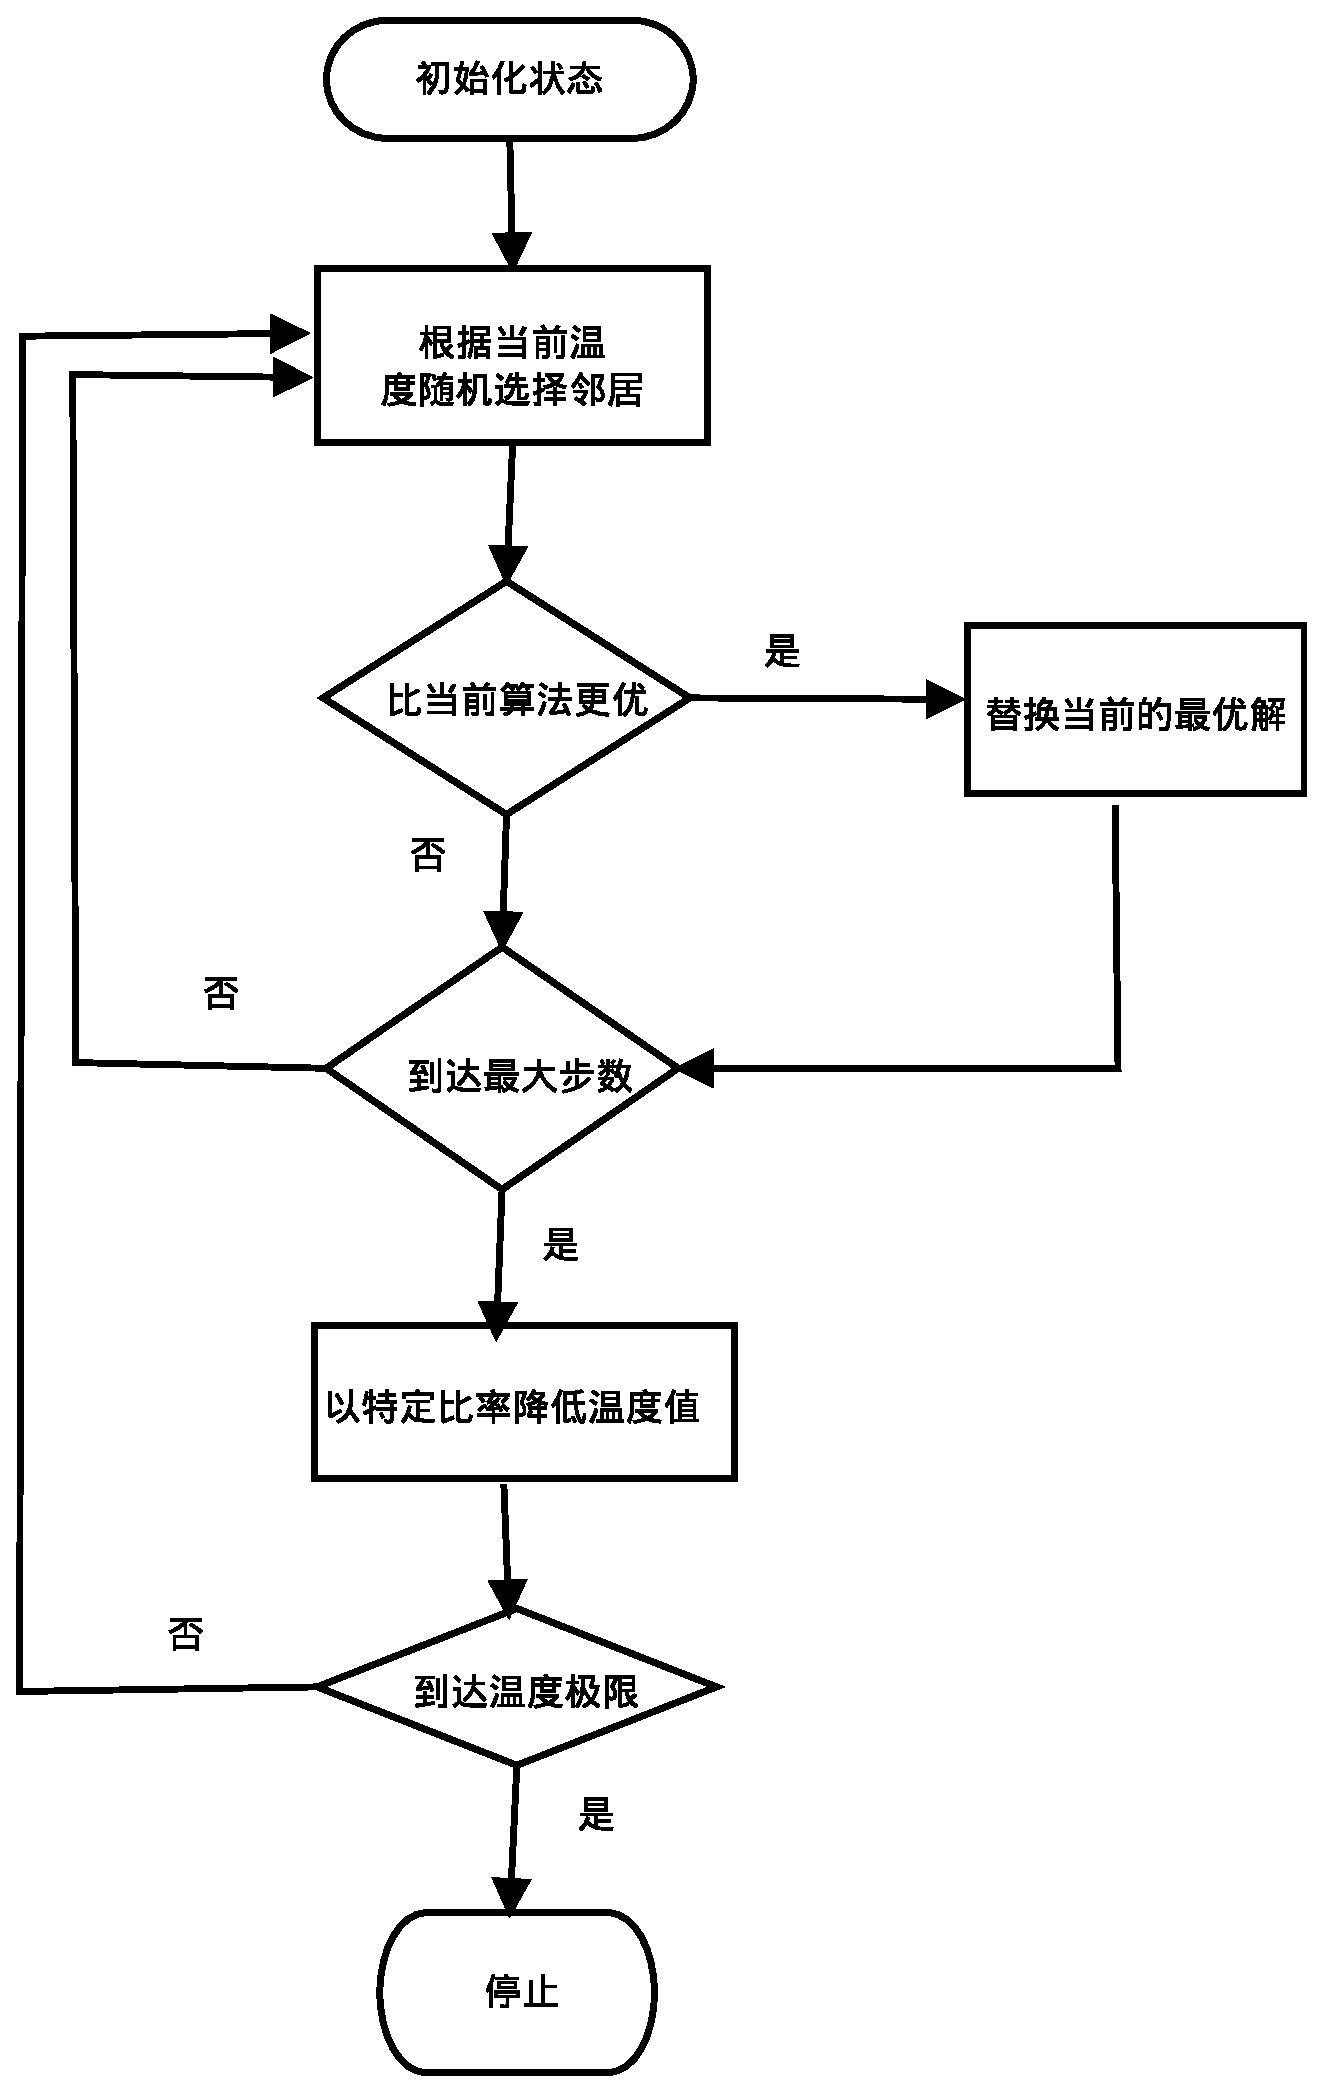
\includegraphics[width=0.6\textwidth]{simulatedannealing}
\caption{模拟退火算法流程图}\label{fig:simulatedannealing}
\vspace{\baselineskip}
\end{figure}
% 基于退火算法的并行算法能够应用在许多组合优化问题上.大部分并行算法可以分为两种形式:(1)函数
%并行,使用多个计算核心来计算每一个步骤的不同阶段(2)数据并行,使用不同的计算节点或者各种不同
%的计算各个不同的步骤.第二种数据并行方法具有"能够轻松通过扩展处理器的数目来增强算法"的优势


\section{旅行售货商问题}
    模拟退火算法算法可以用来解决旅行售货商(Travelling Salesman Problem)问题:设有n个城市,从1,\ldots,n。城市之间有一定的距离
,城市i和城市j之间的距离为D(i,j),其中$i,j=1,\ldots,n$,目的是访问每个城市恰好一次回路,使得旅行总路径的长度最短。旅行售货商
问题属于NP完全问题,为了求解精确的解,必须穷举所有的城市旅行路径,所以时间复杂度为$O(N!)$。模拟退火算法可以用较短时间求出
近似的最优解\cite{Xuzhihong}。

\subsection{旅行售货商算法}
    模拟算法的求解目的为寻找目标函数的最小值。其中,旅行售货商的解空间:为每个城市恰好走一次的所有回路,即所有的城市的排列构成的集合,$S={W_1,W_2,\ldots,W_n}$,初始解选择$W_1$
    目标函数即为走遍所有城市之后总计的长度\cite{},为

    $$F(W_1,W_2,\ldots,W_n)=\sum_{j=1}{n}{W_j,W_{j+1}}$$

在产生每个新解时可以使用多种遍历方法,常用的有1: 随机选择两个结点,交换路径中两点的顺序 2:随机选择两个结点,将路径中个结点见的结点顺序
逆转 3 随机选择3个结点m,n,k,将结点m,n置于结点k之后,详细描述如下:
    
在所有城市中随机选择任意两个城市,进行路径变换形成新的路径:假设初始解空间为${W_1,W_2,\ldots,W_n}$初始路径选择, 如随机产
生1,n城市之间任意两个数k,m ,若$k<m$,则将$$(W_1,W_2,\ldots,W_k,W_{k+1},\ldots,W_m,\ldots,W_n)$$变为$$(W_1,W_2,\ldots,W_m,W_{m-1},\ldots,W_{k+1},W_k,\ldots,W_n) $$
    否则,将$$(W_1,W_2,\ldots,W_k,W_{k+1},\ldots,W_m,\ldots,W_n)$$变为$$(W_m,W_{m-1},\ldots,W_1,W_{m+1},\ldots,W_{k-1},W_n,W{n-1},\ldots,W_k)$$
    转变后的解为$(U_1,U_2,\ldots,U_n)$,前一重方法称为交换算法,后一种算法称为置逆方式,还有一种方式为移位:随机选择两个城市,
将两个城市之间的城市统一右移一位。如随机选出城市k,m($k<m$),则将原路径
$$W_1,W_2,\ldots,W_{k-1},W_k,W_k{k+1},\ldots,W_{m-1},W_m,W_{m+1},\ldots,W_n$$变为新的路径
$$W_1,W_2,\ldots,W_{k-1},W_{m+1},W_k,W_{k+1},\ldots,W_{m-1},W_m,W_{m+2},\ldots,W_n$$
    
代价函数差用来区分新解和原解之间的差别,值为:
    $$\Delta f =f(U_1,U_2,\ldots,U_n)-f(W_1,W_2,\ldots,W_n)=\sum_{j=1}{n}d(U_j,U_{j+1}) - \sum_{j=1}{n}d(W_j,W_{j+1})$$

    本文中模拟退火并行算法采用主从式并行模式,包括主结点在内的计算结点完成SA算法结算,其中主进程决策是否接受或者否决一个解决
方案,同时负责其他子结点的同步。并行模拟退火算法可以有2种策略:
    \begin{itemize}
    \item 每个子结点运行独立的SA算法,所以产生的司机数目也是不同的,相互之间并没有进程的通信。当算法结束时挑选所有子结点中最好的解
    \item 子结点需要和主结点进行通信,返回当前他们的最佳解。这种情况下,当温度太高时,通信量会很多,通信消耗的时间可能大于并行
        带来的时间损耗。
    \end{itemize}
    
    本文采用两者的结合,即在温度很高的时候所有的结点计算都是独立的,只有当温度较低时才会有通信过程。
当温度较低时,采用主从结构-子结点计算出自己的解,将自己的解发送到主结点,主结点判断是否接受,如果接受则将此解广播至各个子结点
。整个主从结点在各个温度阶段独立计算,采用不同步的方式,但是在得到计算结果之后主结点采用同步的方式来获取各个子结点的计算结果。
这样能够保证所有的结点在同样的温度和同样的时间情况下完成计算。 整个算法结束时获得近似最优解。

结点之间的通信计划如下图~\ref{fig:sa}:

    \begin{figure}[htbp]
    \centering
    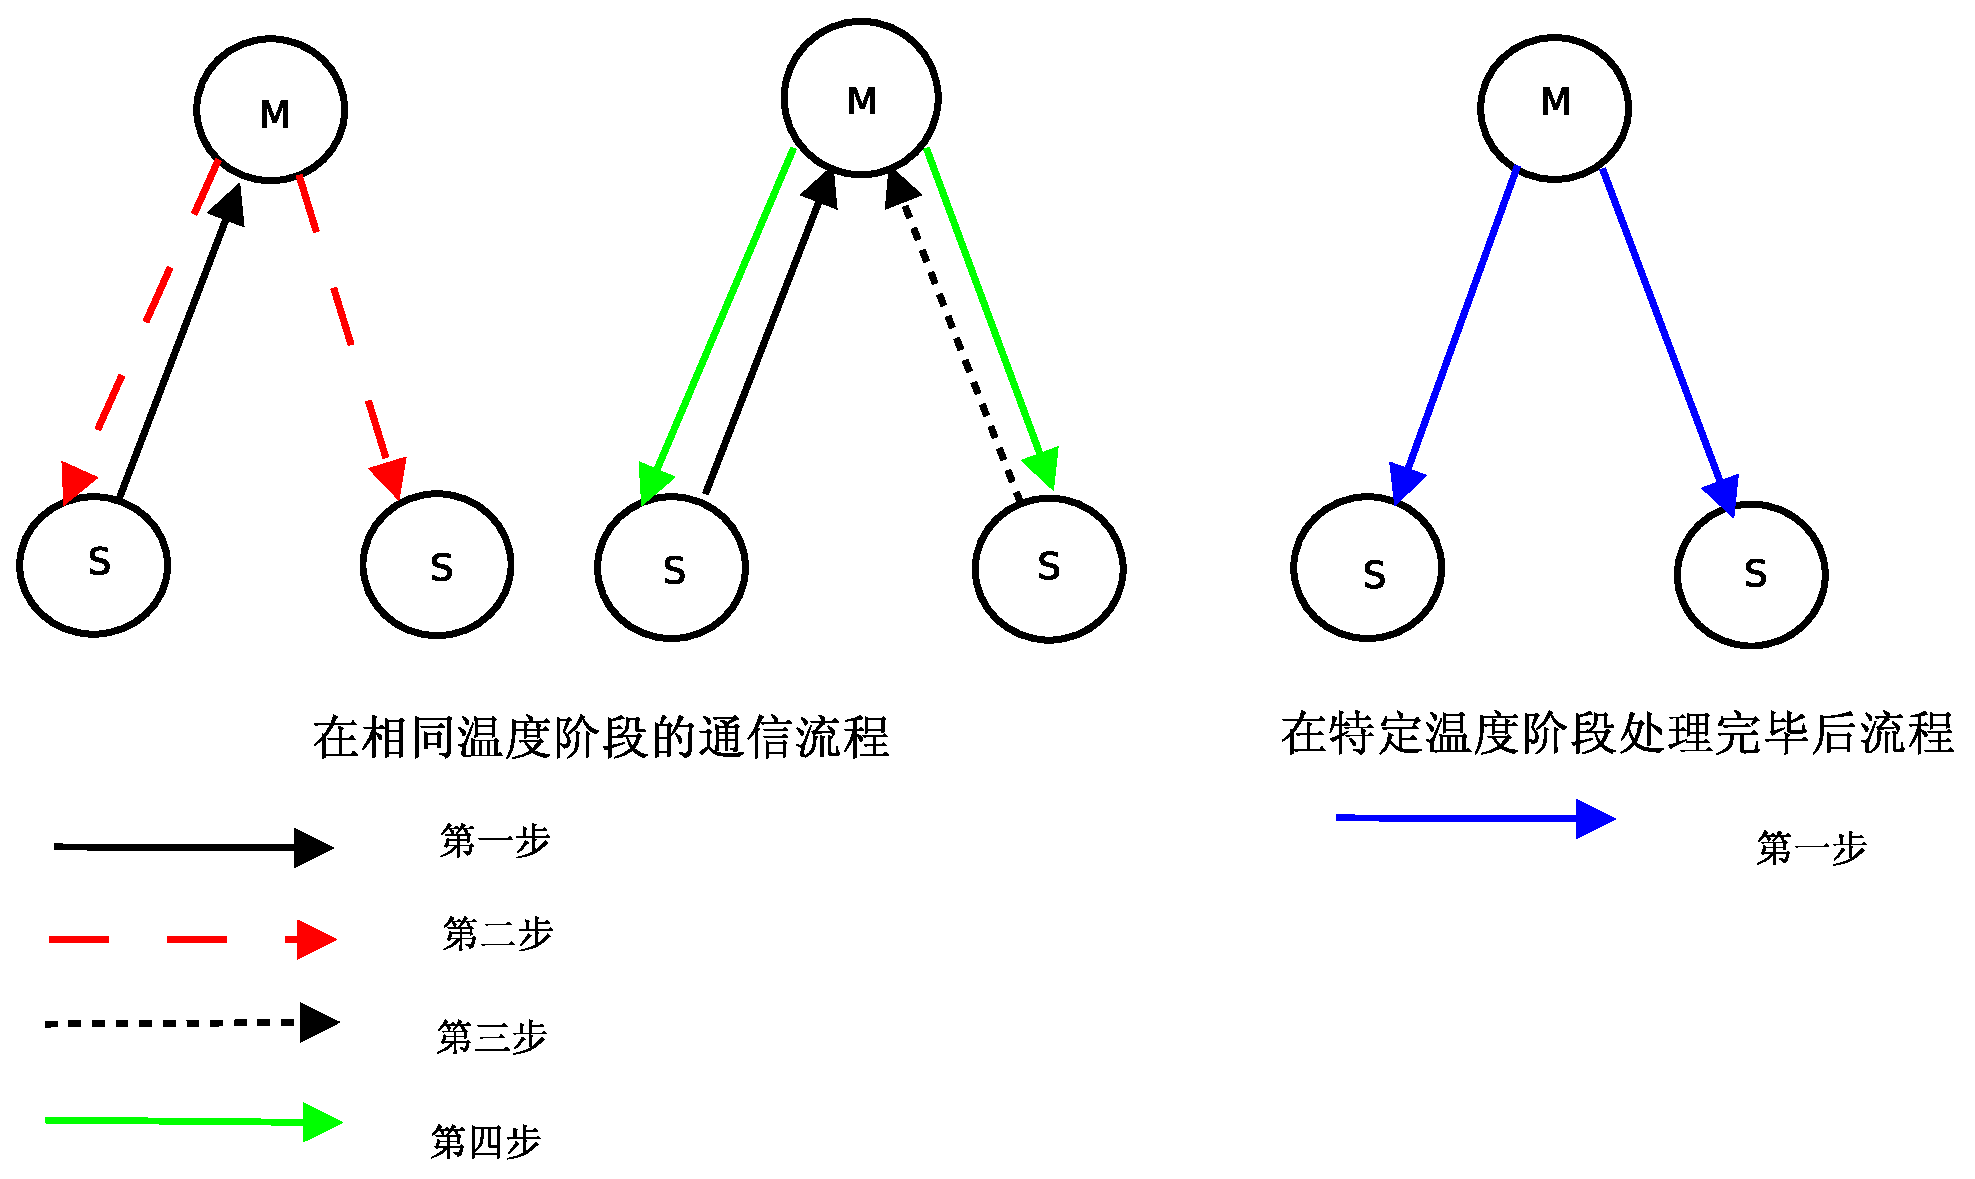
\includegraphics[width=0.9\textwidth]{sa}
    \caption{通信流程}\label{fig:sa}
    \vspace{\baselineskip}
    \end{figure}
    
    只有在特定温度阶段结束后,子进程才与主进程通信。这样所有的进程都几乎在同时通信,没有必要显式的进行同步操作。同时,在一定次数
的迭代之后才进行通讯,同样可以保证进程之间的同步。

    使用模拟退火并行算法解决TSP问题的算法步骤如下,
    \begin{enumerate}
        \item 产生新的路径$S_new$,计算长度$L(S_new)$
        \item 如果产生的路径长度$L(S_new)<L(S)$,则$S=S_new$,将新的路径解决方案设置为当前的路径方案,否则以以下概率
            $$random < min[1,e^{-\frac{f(x^{'}-f(x)}{T}}]$$
            接受新的$S_new$路径,然后步数+1
        \item 重复前两步,直至步数达到终点或者路径长度不再发生变化。
    \end{enumerate}

\subsection{并行算法伪代码}
    模拟退火算法的伪代码.从$S0$状态开始算法,直到到达了$k_{max}$最大步数限制,或者无法获取更大的$F$。新路径的产生使用generate()函数,代价函数差用来比较区别。

算法伪代码如下:
\algrenewcommand{\algorithmiccomment}[1]{\hskip3em$\rightarrow$ #1}
\begin{algorithmic}[1]
\State $S \gets {1,\ldots,n} ; F \gets F(0)$
\Comment  初始化长度和解空间
\State $Sbest \gets S ;Fbest \gets F$
\Comment  初始化最优解
\State $k \gets 0,termination=false$
\Comment  初始化步长
\While {$k < kmanx$ and $termination$}
\For{$1 \gets L$}
    \State $generate(S_new ,S)$
    \Comment $generate new resoluton$
    \State $\Delta t = F(S_new)-F(S)$
    \If {$\Delta < 0 || EXP(-\Delta/T)>Random[0,1]$}
        \State $S=S_new$
    \EndIf
\EndFor
\EndWhile
\State $return S$
\Comment 返回最低的能量状态
\end{algorithmic}


    
\subsection{实验结果}
    将并行后的算法应用在TSP数据库中的city31,att48,对各个数据库进行10此实验求解平均数,可的下表的数据:
    \begin{table}[htbp]
    \centering  % 表居中
    \begin{tabular}{ccccccc}  % {lccc} 表示各列元素对齐方式,left-l,right-r,center-c
    \hline
    问题规模&已知最优解&处理机台数&取得最优解&平均运行时间/s&加速比&并行效率\\ \hline 
    31&15404&1&15416&15.506&1&1\\        
    31&15404&2&15413&8.006&1.93&0.96\\        
    31&15404&4&15414&4.506&3.62&0.90\\        
    48&33525&1&33804&90.257&1&1\\        
    48&33525&2&33794&48.795&1.849&0.911\\        
    48&33525&4&33784&24.402&3.698&0.935\\        
    76&108159&1&110375&440.981&1&1\\        
    76&108159&2&110297&233.688&1.886&0.951\\        
    76&108159&4&110312&120.989&3.644&0.914\\        
    \end{tabular}
    \caption{并行模拟退火算法实验结果}
    \end{table}
    
    加速比等于单机处理时间/多机处理时间,所得结果如下图:
\begin{tikzpicture}
\begin{axis}[
xlabel=处理器的数目,
ylabel=加速比,
height=9cm,
width=9cm,
grid=major,
]
\addplot coordinates {
(1,1)
(2,1.9)
(3,2.9)
(4,3.85)
(5,4.8)
(6,5.6)
(7,6.4)
(8,7.6)
};
\end{axis}
\end{tikzpicture}

综上可见,相对于串行算法来说,并行算法的时间效率大大提高,但模拟退火算法的时间复杂度高,随着并行处理机数目的增加,算法的
并行效率也有所下降。总体来讲,模拟退火算法易受多个参数的影响,有初始值的设置,当初始值过大时,容易获取全局最优解,但是
算法耗时过长,当设置过小时,可能获取局部最优解,无法获取全局最优解。还有退火的迭代量,迭代量太大容易导致时间消耗过大等等。

%http://en.wikipedia.org/wiki/Simulated_annealing
%http://blog.csdn.net/lalor/article/details/7688329
